\chapter{Systemarkitektur}

 
Følgende afsnit indeholder SysML BDD og IBD. BDD'et giver overblik over systemets hardwareblokke samt hvilke inputs og outputs hver blok indeholder. IBD'et viser forbindelserne mellem hardwareblokkene samt hvilken vej kommunikationen foregår.


\section{Block Definitions Diagram}
\noindent Figur~\ref{fig: BDD} viser et Block Definitions Diagram (BDD) over systemet. Det er med for, at give det første overblik over systemet -- altså hvad systemet består af.

Systemet består af fire hardware blokke -- et Inputfilter, et Power-modul, en PWM-forsyning samt et PWM-modul.
Inputfilteret bruges til at filtrere støj, der kommer fra inputkilden, og sikrer dermed en stabil inputspænding. Derudover skal det også filtrere støjsignaler, der kan løbe tilbage til kilden.
Power-modulet består af selve convertertrinet. Det er i denne blok inputspændingen bliver konverteret om til den korrekte udgangsspænding.
PWM-forsyningen står for at forsyne PWM-modulet. Under opstart vil blokken regulere converterens inputspænding ned til den korrekte spænding på 12V. Converterens output vil bruges, når outputspændingen er tilstrækkelig.
PWM-modulet står for selve reguleringen af converterens output. Dette sker ved at overvåge både outputspændingen samt peak-strøm i power-modulet, og tilpasse PWM-signalets duty-cycle herefter.   

\begin{figure}[H]
	\centering
	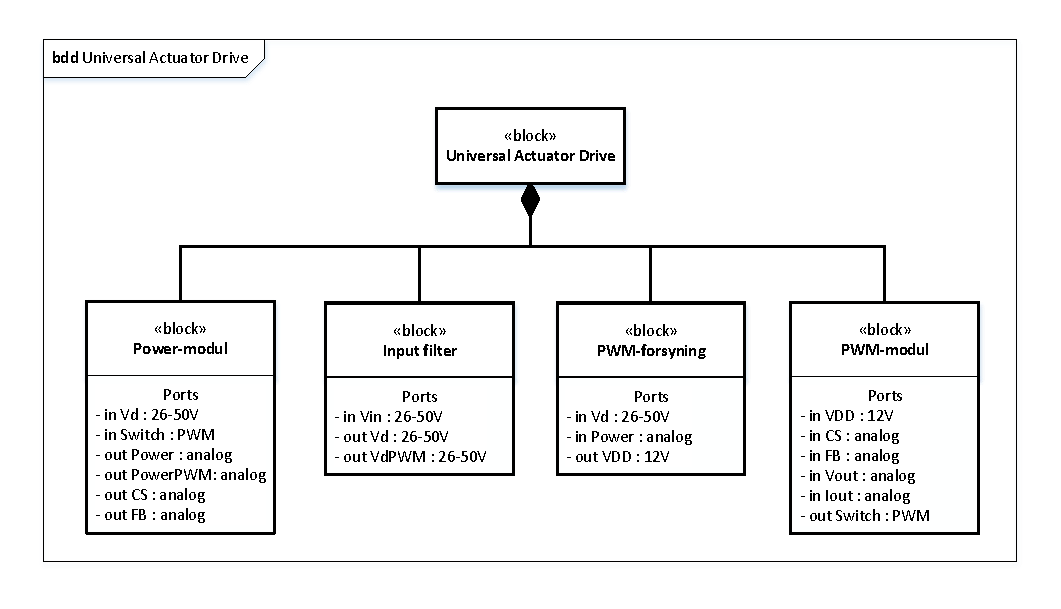
\includegraphics[width=1.00\textwidth]{tex/systemarkitektur/billeder/BDD.pdf}
	\caption{BDD}
	\label{fig: BDD}
\end{figure}

\section{Internal Block Diagram}
\noindent Figur~\ref{fig: IBD} viser et Internal Block Diagram (IBD) over systemet. Dette er skridtet efter BDD'et, og viser hvordan systemets blokke er forbundet.


\begin{figure}[H]
	\centering
	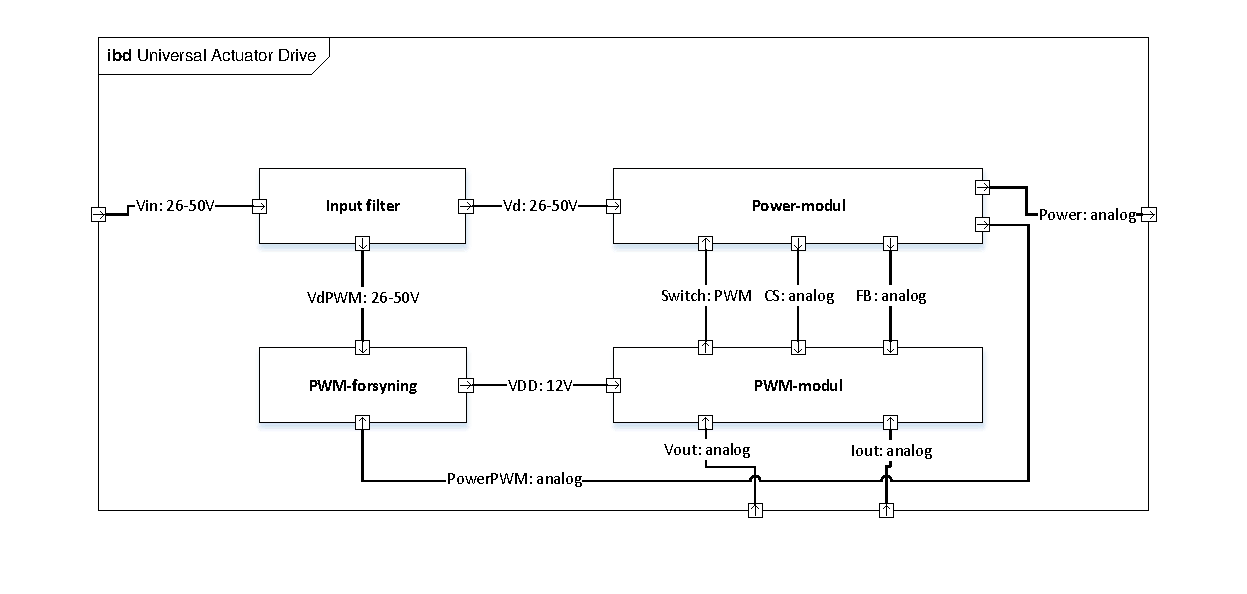
\includegraphics[width=1.00\textwidth]{tex/systemarkitektur/billeder/IBD.pdf}
	\caption{IBD}
	\label{fig: IBD}
\end{figure}


\subsection{Signalbeskrivelse}
\noindent Tabel~\ref*{tabel: Signalbeskrivelse} viser en signalbeskrivelse for systemet. Tabellen indeholder signalets type, navn, og en beskrivelse af signalet.

\begin{table}[htbp]
	\centering
	\begin{tabular}{|l|l|l|}
		\hline
		\textbf{Signal type} 	&\textbf{Navn}		&\textbf{Beskrivelse} \\\hline
		26-50V			&Vin		&Ufiltreret inputspænding på 26-50V\\\hline
		26-50V			&Vd			&filtreret inputspænding på 26-50V\\\hline
		26-50V			&VdPWM			&Input til convertering af PWM-controllerens VDD (under opstart)\\\hline
		15-21V			&PowerPWM		&Input til convertering af PWM-controllerens VDD (efter opstart)\\\hline
		12V				&VDD		&12V forsyning til PWM-controller\\\hline
		15-21V			&Power		&Converterens outputspænding\\\hline
		PWM				&Switch		&PWM signal til regulering af outputspænding\\\hline
		analog			&CS			&Analogt signal til monitorering af peak-strøm   \\\hline	
		analog			&FB			&Analogt signal til monitorering af outputspænding\\\hline
		Vout			&analog		&0-5V signal, som sætter ønsket udgangsspænding\\\hline
		Iout			&analog		&0-5V signal, som sætter ønsket udgangsstrøm\\\hline
		
	\end{tabular}
	\caption{Signalbeskrivelse}
	\label{tabel: Signalbeskrivelse}
\end{table}

